% CHANGES TO THE MAIN TEXT (main__3_.tex), in order of appearance
% Each block below gives WHERE (location + exact anchor text in your file) and WHAT (mode + text).
% This file is an insertion guide and is not meant to be compiled on its own.

%============================================================================================
% [M1a] Abstract: insert after the sentence ending 'under an idealized shift model.'
% ANCHOR: including its boundary-induced attenuation under an idealized shift model.
% MODE:   insert AFTER the anchor
%============================================================================================
 Building on the envelope gradients, we derive exact gradients of the debiased state discrepancy, of anomaly scores, of the doubly debiased trajectory discrepancy and of the level-adjusted lead--lag index, the last as a covariance under the Gibbs distribution over alignment paths, and bound the error of first-order predictions.

%============================================================================================
% [M1b] Abstract: append at the end (after 'the most structurally distinctive year.')
% ANCHOR: 2020 is not the most structurally distinctive year.
% MODE:   insert AFTER the anchor
%============================================================================================
 About 3\% of the directed corridors, centred on the largest hubs, carry half of the local sensitivity of each annual anomaly score; targeted changes of at most 50\% to 4\% of the 2020 corridor costs would make 2020 the most distinctive year, whereas an across-the-board increase of 25\% would not.

%============================================================================================
% [M1c] Keywords: replace
% ANCHOR: Lead--lag estimation; Optimal transport; Shapley attribution
% MODE:   REPLACE the anchor with
%============================================================================================
Lead--lag estimation; Optimal transport; Sensitivity analysis; Shapley attribution

%============================================================================================
% [M2a] Introduction, list of contributions: insert a new item before the item 'Evidence'
% ANCHOR: \item \emph{Evidence.}
% MODE:   insert BEFORE the anchor
%============================================================================================
\item \emph{Sensitivity.} Exact gradients of the debiased discrepancy, which must account for both arguments of the self-comparison; of anomaly scores and of the doubly debiased G-STA discrepancy, in which state-level gradients are weighted by expected alignment frequencies; and of the level-adjusted lead--lag index, through covariances of the Gibbs distribution over alignment paths. A frozen-coupling bound controls the error of first-order predictions of state-level values, and budgeted counterfactual perturbations are evaluated by full re-optimization (Propositions~\ref{prop:graddelta}--\ref{prop:local}).

%============================================================================================
% [M2b] Introduction, item 'Evidence': replace
% ANCHOR: Verification against explicit tensors, exhaustive path enumeration and finite differences;
% MODE:   REPLACE the anchor with
%============================================================================================
Verification against explicit tensors, exhaustive path enumeration and re-solved finite differences, including the new gradients;

%============================================================================================
% [M2c] Introduction, item 'Evidence': replace the end of the item
% ANCHOR: an exploratory application to bilateral transport costs among 86 economies.
% MODE:   REPLACE the anchor with
%============================================================================================
an exploratory application to bilateral transport costs among 86 economies, with influence measures and counterfactual stress tests.

%============================================================================================
% [M2d] Introduction, roadmap sentence: replace
% ANCHOR: Section~\ref{sec:temporal} the temporal layer,
% MODE:   REPLACE the anchor with
%============================================================================================
Section~\ref{sec:temporal} the temporal layer and its sensitivity analysis,

%============================================================================================
% [M3] Section 3.4 (Envelope gradients), paragraph after Proposition 6: replace the last sentence
% ANCHOR: Gradients of~\eqref{eq:delta} follow by the chain rule, accounting for the appearance of the same state in both arguments of a self-term.
% MODE:   REPLACE the anchor with
%============================================================================================
Gradients of~\eqref{eq:delta}, of anomaly scores, of G-STA and of the lead--lag index, and the accuracy of first-order predictions, are derived in Section~\ref{sec:sensitivity}; whether a perturbation changes the selected branch is checked by re-solving.

%============================================================================================
% [M4] NEW Section 4.5: insert at the end of Section 4 (after Subsection 4.4 'Summaries of a single trajectory'), before \section{Numerical studies}
% ANCHOR: \section{Numerical studies}
% MODE:   insert BEFORE the anchor
%============================================================================================
\subsection{Gradient-based sensitivity of network trajectories}\label{sec:sensitivity}

Proposition~\ref{prop:envelope} differentiates the value of one branch of stationary points. The quantities reported in practice are debiased portfolio estimates and, for trajectories, pass through soft alignment. The free inputs of a state $G$ are the observed relations $c_{ik}$ ($i\neq k$, $w_{ik}>0$), the attributes and the masses; masks are held fixed, because a change of observation status is a discrete change of the objective (Corollary~\ref{cor:mask}). For a pair $(G,H)$ we write $\partial_1V$ and $\partial_2V$ for the formulas of Proposition~\ref{prop:envelope} with respect to the inputs of the first and of the second argument, evaluated at the selected coupling.

\begin{definition}[Regular selection]\label{def:regular}
The selection is \emph{regular} at $(G,H)$ if, in a neighbourhood of the inputs, every candidate of the portfolio that attains $\widehat V_\varepsilon(G,H)$ follows the continuously differentiable branch of stationary points through a common point $P^\star$ at which $\nabla_P^2J_\varepsilon$ is non-singular.
\end{definition}

Under a regular selection $\widehat V_\varepsilon$ coincides locally with one branch value; where candidates on different branches tie it has a kink and only one-sided derivatives.

\begin{proposition}[Gradient of the debiased discrepancy]\label{prop:graddelta}
Let the selection be regular at $(G,H)$, $(G,G)$ and $(H,H)$, with selected couplings $P$ for $(G,H)$ and $S$ for $(G,G)$, $r=P\mathbf 1$ and $r_S=S\mathbf 1$.
(a) For every free input $x$ of $G$,
$\partial_x\widehat\Delta_\varepsilon(G,H)=\partial_{1,x}\widehat V_\varepsilon(G,H)-\tfrac12\{\partial_{1,x}\widehat V_\varepsilon(G,G)+\partial_{2,x}\widehat V_\varepsilon(G,G)\}$; inputs of $H$ are treated symmetrically.
(b) With the portfolio of Section~\ref{sec:multistart}, $S=S^\top$, the two self-terms coincide, and
\begin{align*}
\nabla_C\widehat\Delta_\varepsilon&=2\alpha\,W\circ\{C\circ(PW'P^\top-SWS)-P(W'\circ D)P^\top+S(W\circ C)S\},\\
\nabla_F\widehat\Delta_\varepsilon&=2(1-\alpha)\{\operatorname{diag}(r-r_S)F-PG+SF\},\qquad
\nabla_\mu\widehat\Delta_\varepsilon=\gamma\,(r_S-r)/\mu .
\end{align*}
(c) If $H$ is a copy of $G$, $\nabla\widehat\Delta_\varepsilon(G,H)=0$, whereas the gradient $\partial_1\widehat V_\varepsilon(G,G)$ of the raw value is non-zero in general.
\end{proposition}

The mass sensitivity of the debiased discrepancy compares how much of a node's mass the cross-coupling and the self-coupling transport; the raw value adds the entropic bias $\gamma(\mathbf 1-r_S/\mu)$, which is present even when $H=G$.

\begin{proposition}[Gradients of trajectory summaries]\label{prop:gradgsta}
Let $x$ be a free input of the state $G_t$ of $\mathcal G$, let all selections involving $G_t$ be regular, and write $\nabla_x\Delta_{tu}=\partial_x\widehat\Delta_\varepsilon(G_t,G_u)$ and $\nabla_x\Delta^{\mathcal{GH}}_{ts}=\partial_x\widehat\Delta_\varepsilon(G_t,H_s)$.
(a) $\partial_xa(t)=(T-1)^{-1}\sum_{u\neq t}\nabla_x\Delta_{tu}$ and, for $u\ne t$, $\partial_xa(u)=(T-1)^{-1}\nabla_x\Delta_{tu}$.
(b) For fixed $\beta$, with $E^{\mathcal{GH}}=\nabla\mathcal A_\beta(\Delta^{\mathcal{GH}})$ and $E^{\mathcal{GG}}=\nabla\mathcal A_\beta(\Delta^{\mathcal{GG}})$,
\[
\partial_x\widehat{\mathrm{GSTA}}(\mathcal G,\mathcal H)=\sum_{s=1}^{S}E^{\mathcal{GH}}_{ts}\nabla_x\Delta^{\mathcal{GH}}_{ts}-\sum_{u\neq t}E^{\mathcal{GG}}_{tu}\nabla_x\Delta_{tu}.
\]
(c) If $\mathcal H$ is a copy of $\mathcal G$, the gradient in (b) vanishes.
\end{proposition}

The weights are expected alignment frequencies (Proposition~\ref{prop:sdtw}(c)): a relation that strongly affects $\Delta(G_t,H_s)$ for rarely aligned periods has little influence on the trajectory comparison, and the self-alignment term removes the part of its influence shared with the other periods of its own trajectory. With $\beta$ set from the data as in Section~\ref{sec:temporal}, (b) acquires the term $(\partial\widehat{\mathrm{GSTA}}/\partial\beta)\,\partial_x\beta$, where $\partial\mathcal A_\beta(\Delta)/\partial\beta=\{\mathcal A_\beta(\Delta)-\langle E,\Delta\rangle\}/\beta=-H(p_\beta)$ is minus the entropy of the Gibbs distribution over paths; we hold $\beta$ at its observed value.

\begin{proposition}[Gradient of the lead--lag index]\label{prop:gradll}
Let $Z=\sum_{ts}E_{ts}=\mathbb E_\beta|A|$ and let $Y(A)=\sum_{(t,s)\in A}(s-t-\tau)$ be the excess offset of a path.
(a) For fixed $\beta$, $\nabla_\Delta\tau=-(\beta Z)^{-1}\operatorname{Cov}_\beta(Y,A)$, and $|\partial\tau/\partial\Delta_{ts}|\le\operatorname{sd}_\beta(Y)/(2\beta Z)$.
(b) Let $\hat\tau$ be computed from $\tilde\Delta=\Delta-\min\Delta$ with $\beta=b\operatorname{med}(\tilde\Delta)$. Where the minimizing cell $k^\star$ and the cells defining the median are unique, $\hat\tau$ is differentiable,
$\nabla\hat\tau=g-\langle g,\mathbf 1\mathbf 1^\top\rangle e_{k^\star}-\{\langle g,\tilde\Delta\rangle/\operatorname{med}(\tilde\Delta)\}(\bar e_{\mathrm{med}}-e_{k^\star})$,
with $g$ the gradient in (a) at $\tilde\Delta$ and $\bar e_{\mathrm{med}}$ the (averaged) indicator of the median cell(s); moreover $\langle\nabla\hat\tau,\mathbf 1\mathbf 1^\top\rangle=\langle\nabla\hat\tau,\Delta\rangle=0$ and $\nabla\hat\tau(\Delta^\top)=-\nabla\hat\tau(\Delta)^\top$.
(c) Under regular selections, for a free input $x$ of $G_t$, $\partial_x\hat\tau(\mathcal G,\mathcal H)=\sum_s(\nabla\hat\tau)_{ts}\nabla_x\Delta^{\mathcal{GH}}_{ts}$.
\end{proposition}

Raising $\Delta_{ts}$ lowers $\tau$ exactly when paths through $(t,s)$ have above-average excess offset. As $\beta\to0$ with a unique optimal path the covariance vanishes and $\tau$ becomes locally constant: timing sensitivity is a finite-temperature property of the soft alignment. Since $\nabla^2\mathcal A_\beta=-\beta^{-1}\operatorname{Cov}_\beta(A)$, Hessian--vector products cost $O(TS)$ by forward differentiation of the soft-DTW recursions.

\begin{proposition}[Accuracy of first-order predictions]\label{prop:local}
(a) Let $P$ be any coupling and $\delta=(\delta C,\delta F,\delta\mu)$ a perturbation of the free inputs of $G$ with $\mu+\delta\mu>0$. The global optimum and the value $V^{\mathrm{bf}}$ returned by Algorithm~\ref{alg:gcg} started at $P$ for the perturbed pair satisfy
$V_\varepsilon(G+\delta,H)\le V^{\mathrm{bf}}\le J_\varepsilon(P)+\langle\partial_\theta J_\varepsilon(P),\delta\rangle+R_P(\delta)$, where
\[
R_P(\delta)=\alpha\sum_{ik}w_{ik}(PW'P^\top)_{ik}\delta c_{ik}^2+(1-\alpha)\sum_ir_i\|\delta f_i\|^2+\gamma\sum_ir_i\Bigl\{\tfrac{\delta\mu_i}{\mu_i}-\log\Bigl(1+\tfrac{\delta\mu_i}{\mu_i}\Bigr)\Bigr\}\ge0;
\]
at the selected coupling $J_\varepsilon(P)=\widehat V_\varepsilon(G,H)$ and $\partial_\theta J_\varepsilon(P)$ is the envelope gradient.
(b) Let $\mathcal S$ be $\widehat\Delta_\varepsilon$, $a(t)$, $\widehat{\mathrm{GSTA}}$ or $\hat\tau$, and $\theta_\lambda=\theta_0+\lambda\delta$. If for $\lambda\in[0,1]$ all selections are regular and remain on the branches through $\theta_0$, and the cells of Proposition~\ref{prop:gradll}(b) do not change, then $\mathcal S$ is twice continuously differentiable on the segment and
$|\mathcal S(\theta_1)-\mathcal S(\theta_0)-\nabla\mathcal S(\theta_0)^\top\delta|\le\tfrac12\max_\lambda|\delta^\top\nabla^2\mathcal S(\theta_\lambda)\delta|$.
(c) For weights $q_k>0$ and bounds $\bar u_k$, the problem $\max_u\pm\langle\nabla\mathcal S,u\rangle$ subject to $\sum_kq_k|u_k|\le B$ and $|u_k|\le\bar u_k$ is solved by ranking coordinates by $|\partial_k\mathcal S|/q_k$ and setting $u_k=\pm\operatorname{sign}(\partial_k\mathcal S)\bar u_k$ in that order until the budget is exhausted, the last coordinate fractionally.
\end{proposition}

Part (a) holds for every perturbation, not only small ones: re-optimizing the coupling can only lower a cross-term below its frozen-coupling prediction. In $\widehat\Delta_\varepsilon$ the self-term enters with the opposite sign, so first-order predictions of debiased quantities are not one-sided, in line with Proposition~\ref{prop:optimization-error}. Because (b) fails where the selection changes branch, every perturbation is evaluated by re-solving all affected problems with the portfolio and, separately, by following the original branch.

\emph{Influence measures.} For a summary $\mathcal S$ and a perturbation scale $\sigma_{ik}$, the standardized sensitivities $\tilde g_{ik}=\sigma_{ik}\partial\mathcal S/\partial c_{ik}$ define outgoing, incoming and total influence $S_i^{\mathrm{out}}=\sum_{k\neq i}|\tilde g_{ik}|$, $S_i^{\mathrm{in}}=\sum_{k\neq i}|\tilde g_{ki}|$, $S_i=S_i^{\mathrm{out}}+S_i^{\mathrm{in}}$, and the directional imbalance $B_i=(S_i^{\mathrm{out}}-S_i^{\mathrm{in}})/(S_i+\eta)$. For a pair observed in both directions, the derivatives along $\delta(E_{ik}+E_{ki})$ and $\delta(E_{ik}-E_{ki})$ are $D_S=g_{ik}+g_{ki}$ and $D_A=g_{ik}-g_{ki}$; the antisymmetric share $\sum D_A^2/\sum(D_S^2+D_A^2)$ is the sensitivity counterpart of Proposition~\ref{prop:decomp}. The split measures mismatch at a fixed coupling; the gradient measures how the optimized discrepancy responds. If the inputs carry independent errors with standard deviations $\sigma_{ik}$, the delta method gives $\operatorname{Var}\mathcal S\approx\sum_{ik}\tilde g_{ik}^2$, a local approximation whose accuracy we check by simulation in Section~\ref{sec:influence}.

%%%%%%%%%%%%%%%%%%%%%%%%%%%%%%%%%%%%%%%%%%%%%%%%%%%%%%%%%%%%%%%%%%%%%%%%%%%%%%

%============================================================================================
% [M5a] Table 1 (tab:verif): add rows after the last row, before \bottomrule
% ANCHOR: $\alpha=0$ vs.\ POT \texttt{sinkhorn\_unbalanced}; soft-DTW vs.\ enumeration (max.\ errors) & $5.7\times10^{-12}$; $4.0\times10^{-15}$\\
% MODE:   insert AFTER the anchor
%============================================================================================
Debiased gradient (Prop.~\ref{prop:graddelta}) vs.\ re-solved central differences (max.\ rel.\ error, 24 blocks) & $7.5\times10^{-6}$\\
\quad omitting the second self-argument; raw value instead of debiased (rel.\ error) & 0.06--0.25; 0.12--0.49\\
\quad derivative with respect to an unobserved relation & 0\\
Anomaly, G-STA and lead--lag gradients (Props.~\ref{prop:gradgsta}--\ref{prop:gradll}) vs.\ re-solved differences (max.\ rel.\ error) & $8.6\times10^{-6}$\\
Soft-DTW Hessian--vector products vs.\ enumeration; $\nabla\hat\tau$ vs.\ central differences & $8.3\times10^{-15}$; $1.7\times10^{-11}$\\
Data: gradients of $\Delta$, $a(2020)$, G-STA and $\hat\tau$ vs.\ re-solved differences (max.\ rel.\ error, costs) & $9.2\times10^{-6}$\\
Frozen-coupling bound (Prop.~\ref{prop:local}(a)), 72 perturbations: largest excess & $-7.8\times10^{-10}$\\
Re-solved perturbed problems that changed branch (of 1{,}680) & 0\\

%============================================================================================
% [M5b] NEW Section 5.5: insert at the end of Section 5 (after Subsection 5.4 'Missing edges' and Table 3), before \section{An exploratory application...}
% ANCHOR: \section{An exploratory application
% MODE:   insert BEFORE the anchor
%============================================================================================
\subsection{Verification of the sensitivity formulas}\label{sec:verifsens}

We compared Propositions~\ref{prop:graddelta}--\ref{prop:gradll} with central differences (step $10^{-5}$) in which every affected state-level problem is re-solved with the full portfolio to a gap of $10^{-13}$. We used four instance types: a directed instance; a directed instance with 25\% missing relations; networks with 8 and 6 nodes and 20\% missing relations; and a near copy. For both arguments and every block, the gradient of Proposition~\ref{prop:graddelta} agrees to a relative error of at most $7.5\times10^{-6}$. In the near copy the feature gradients are of order $10^{-6}$ and agree to $7\times10^{-11}$ in absolute terms (Table~\ref{tab:verif}; Supplement Table~S12). Two shortcuts fail. Omitting the second argument of the self-comparison gives relative errors of 6\%--25\%, and differentiating the raw value instead of the debiased discrepancy gives 12\%--49\%. Near a copy, where the debiased gradient almost vanishes (Proposition~\ref{prop:graddelta}(c)), the raw gradient is 237 times too large. Derivatives with respect to unobserved relations are exactly zero.

For trajectories of five states with 8 and 6 nodes and 15\% missing relations, the gradients of the anomaly score (with respect to the state's own inputs and to those of another state), of the doubly debiased G-STA discrepancy and of the level-adjusted lead--lag index agree with re-solved differences to a relative error of at most $8.6\times10^{-6}$ (Supplement Table~S13). Soft-DTW Hessian--vector products agree with exhaustive enumeration of all 1{,}683 paths for $T=S=6$ to $8\times10^{-15}$. The smallest eigenvalue of the scaled Hessian $\operatorname{diag}(P)^{1/2}\nabla^2_PJ_\varepsilon\operatorname{diag}(P)^{1/2}$ was at least 0.027 in every instance, so the selected couplings are non-degenerate local minimizers.

Where the selection is not regular, the formulas give one-sided derivatives only. Supplement Figure~S6 follows a path along which two stationary branches, matching two interchangeable nodes in opposite ways, exchange the lead. The portfolio estimate is their lower envelope. Away from the crossing, each branch slope given by Proposition~\ref{prop:graddelta} matches the local slope of the estimate; at the crossing the estimate has a kink, the one-sided slopes differ by 2.05 ($+1.03$ against $-1.03$), and a central difference across it estimates neither. Re-solving with branch following, as we do for every perturbation in Section~\ref{sec:influence}, detects such crossings. Verification on the data is reported in Section~\ref{sec:influence}.

%%%%%%%%%%%%%%%%%%%%%%%%%%%%%%%%%%%%%%%%%%%%%%%%%%%%%%%%%%%%%%%%%%%%%%%%%%%%%%

%============================================================================================
% [M6] Section 6.4 (Regional timing): replace the hard-coded reference
% ANCHOR: Proposition~9(d)
% MODE:   REPLACE the anchor with
%============================================================================================
Proposition~\ref{prop:leadlag}(d)

%============================================================================================
% [M7] NEW Section 6.5: insert at the end of Section 6 (after Subsection 6.4 'Regional timing' and Table 5), before \section{Discussion}
% ANCHOR: \section{Discussion}
% MODE:   insert BEFORE the anchor
%============================================================================================
\subsection{Structural influence and counterfactual perturbations}\label{sec:influence}

We computed the gradients of Section~\ref{sec:sensitivity} at the selected couplings of the main specification, re-solved to a gap of $10^{-12}$. All selections are regular. In each of the 21 year-level problems the three starts converge to the same coupling (largest relative difference $9\times10^{-6}$), and the smallest eigenvalue of the scaled Hessian lies between 0.015 and 0.049. In each of the 540 regional cells all four starts reach the same value. Re-solved central differences agree with the analytic gradients to relative errors of $2\times10^{-6}$ for $\Delta(G_{2020},G_{2021})$ and $1\times10^{-6}$ for $a(2020)$. For the regional G-STA and lead--lag indices of EAP and SSEA the errors are $8\times10^{-6}$ and $9\times10^{-6}$ (Supplement Table~S14). We report derivatives on the scales on which the data are measured. These are \emph{semi-elasticities} $\partial\mathcal S/\partial\log x$ with respect to the cost of a corridor, the LSCI of an economy and its throughput, holding the pooled standardization constants fixed. A 1\% change of $x$ changes $\mathcal S$ by about $0.01\,\partial\mathcal S/\partial\log x$, and winsorized costs have zero semi-elasticity. The \emph{leverage} of a channel, $0.01\sum|\partial\mathcal S/\partial\log x|$, is the first-order change caused by a 1\% change of every input of the channel in its most effective direction.

\emph{Annual anomalies.} Table~\ref{tab:maps} and Figure~\ref{fig:sens} summarize the sensitivity of the anomaly scores. Locally, the three channels are of comparable importance. The leverage of a year's own costs is $7$--$15\times10^{-4}$, about 1\% of $a(t)$, against $3$--$6\times10^{-4}$ for connectivity and $4$--$7\times10^{-4}$ for throughput. This complements the Shapley attribution, which assigns 86\%--98\% of the realized changes to the geometry. Costs move far more from year to year than connectivity or throughput, so most of the realized change is structural even though a unit change of an attribute matters about as much. The costs of the other five years have about the same leverage on $a(t)$ as the year's own costs, because every anomaly score averages comparisons.

Sensitivity is concentrated. About 3\%--4\% of the roughly 6{,}400 observed corridors carry half of the corridor leverage of each year, and 21\%--24\% of the economies carry half of the node influence. The influence $S_i$ of an economy is strongly associated with its mass (Spearman correlations 0.70--0.87). China, Hong Kong SAR is the most influential economy in every year, followed by China and Singapore (Figure~\ref{fig:sens}(a); Supplement Table~S15). The influential corridors are nevertheless spread across the map. Corridors within regions account for only 7\%--9\% of the corridor sensitivity, and the largest blocks are the corridors from East Asia and from South and South-East Asia to Europe (9\% and 7\%; Figure~\ref{fig:sens}(c)). The sensitivity profile is stable from year to year (Spearman correlations between years 0.64--0.75), but the identity of the most influential corridors is not: two years share only 18\%--35\% of their hundred most influential corridors, which reflects the noise in pair-level costs.

The signs are informative. A cost increase would make the year more anomalous on 47\% and 45\% of the corridors in 2016 and 2021, against 28\%--31\% in 2017--2020, in line with the higher cost levels at the ends of the window. Between 39\% and 51\% of the squared corridor gradient lies in the antisymmetric direction. This is close to the 43\%--49\% antisymmetric share of the structural energy, so directional perturbations matter as much locally as in the realized change. The largest sensitivity in 2020, on the corridor from China, Hong Kong SAR to the United Arab Emirates, has the opposite sign to that of the reverse corridor, so the anomaly responds to a reversal of the cost asymmetry on that pair (Supplement Table~S16). Gradients of the raw value $V_\varepsilon$ instead of the debiased discrepancy preserve the ranking of corridors (Spearman correlations of magnitudes 0.95--0.996). However, they misstate magnitudes by 5\%--18\% in norm, and omitting the second self-argument misstates them by half as much.

\emph{Regional trajectories and timing.} Table~\ref{tab:regsens} reports which economies carry the sensitivity of the lead--lag index. First, in comparisons between regions the node attributes dominate local sensitivity. Connectivity carries 66\%--89\% of the leverage of $\hat\tau$, throughput most of the rest, and corridor costs only 1\%--6\%; the same holds for G-STA. Between different node sets the coupling is anchored by attributes and masses, whereas a region contains few corridors. Second, timing and dissimilarity are carried by partly different relations: the Spearman correlation between the corridor sensitivity profiles of $\hat\tau$ and of G-STA is 0.37--0.58. By contrast, the G-STA profile is almost the same as that of the comparison of the same years (median correlation 0.95, minimum 0.85), so allowing the alignment to adjust barely reorders the influence of corridors. Third, the antisymmetric share of the corridor gradient of $\hat\tau$ is 0.26--0.46 (mean 0.37), and it is smaller than that of G-STA in only 6 of the 15 pairs. The closeness of the directed and symmetrized indices in Table~\ref{tab:reg} is therefore a statement about the level of the index, not about its local sensitivity.

The timing signal sits where the alignment is warped. For EAP and SSEA, 86\% of the leverage on the East Asian side comes from its states of 2017--2019, and 49\% on the South-East Asian side comes from its state of 2021. The invariances of Proposition~\ref{prop:gradll}(b) hold on the data to $10^{-12}$. Halving or doubling $\beta$ leaves the sensitivity ranking nearly unchanged (Spearman correlations at least 0.93), but for some pairs it moves the index itself substantially, for SSEA and LAC from 0.06 to 0.66. This is a reminder that six periods support only coarse statements about timing.

\emph{Counterfactual perturbations.} We used the gradients to construct budgeted perturbations of corridor costs. Each perturbation was evaluated by re-solving every affected state-level problem with the portfolio and, separately, by following the original branch. A perturbation $u_{ik}$ is a change of the log cost bounded by $|u_{ik}|\le0.5$ (a factor of 1.65), with budget $B=\sum|u_{ik}|$; the gradient strategy is the solution of Proposition~\ref{prop:local}(c). It is compared with four allocations of the same budget. Three use the signs of the gradient: the heaviest pairs by $\mu_i\mu_k$, randomly chosen corridors, and an equal change of all corridors. They differ from the gradient strategy only in where the budget is spent. The fourth uses the data but not the gradient, moving the corridors with the largest observed cost changes. Perturbed costs are transformed with the baseline winsorization and scaling constants. These exercises are stress tests of the discrepancy, not evaluations of transport policy. We consider three questions (Table~\ref{tab:cf}, Figure~\ref{fig:cf}).

(i) \emph{Which changes of the 2021 costs would most reduce the 2020--2021 structural change?} Changing 16 corridors ($B=8$) reduces $\Delta(G_{2020},G_{2021})=0.093$ by 5\%, and changing 256 corridors ($B=128$) reduces it by 23\%. Undoing the largest observed cost changes achieves 10\% with the same budget, and the other allocations at most 3\%.

(ii) \emph{How robust is the finding that 2020 is not distinctive?} We perturbed the 2020 costs to raise the margin $a(2020)-\max_{t\neq2020}a(t)=-0.025$, which is negative because 2016 leads. The gradient strategy makes 2020 the most distinctive year with 256 corridors, 4\% of the 6{,}429 eligible ones. The mass-weighted allocation needs 2{,}048 corridors, and the cost-change, random and uniform allocations need 4{,}096 or all of them. An across-the-board increase of all 2020 costs leaves 2020 fourth at 5\% and 10\% and third at 25\%. It makes 2020 first only at 50\%, more than ten times the observed increase of the median cost from 2019 to 2020. The conclusion about 2020 is therefore robust to general cost shocks and to untargeted perturbations, but not to large changes concentrated on a few hundred hub corridors. The standard deviation of annual log changes of single-corridor costs, 0.86, exceeds the bound of 0.5, so the conclusion should be read as a statement about the network-wide pattern rather than about every corridor.

(iii) \emph{Could corridor costs remove the alignment lead of East Asia over South and South-East Asia?} We perturbed the SSEA costs of all six years to move $\hat\tau(\mathrm{EAP},\mathrm{SSEA})=0.95$ towards zero. Changing 32 region-year corridors ($B=16$) along the gradient lowers it to 0.77, while the other allocations lower it to between 0.92 and 0.94. Consistent with the dominance of the attribute channel, the timing index is robust to cost perturbations of this size.

First-order predictions were reliable throughout in direction and in the ranking of strategies, but accurate in magnitude only for small budgets. For the reductions in (i), the realized change was 87\% of the predicted change with two corridors and 64\% with 256. For the increases in (ii) it was 125\%--159\% (Supplement Table~S17). Both deviations have the sign implied by the curvature of the re-optimized value: moving a state towards another gains less than linearly, and moving it away gains more. For the index in (iii), which is not a discrepancy, the realized changes were 127\%--187\% of the predicted ones. The frozen-coupling bound of Proposition~\ref{prop:local}(a) held for the cross-term in all 72 perturbations of (i). None of the 1{,}680 re-solved problems changed branch, and the portfolio and branch-following values agreed in every case.

\emph{Uncertainty.} We propagated independent multiplicative errors in the observed costs, with standard deviation $\sigma_m$ on the log scale, through the delta method of Section~\ref{sec:sensitivity}. The resulting standard deviations of the anomaly scores are $5$--$7\times10^{-4}$ for $\sigma_m=0.1$ and $1.2$--$1.7\times10^{-3}$ for $\sigma_m=0.25$. In 12 Monte Carlo replications per level, each re-solving all 21 problems, the empirical standard deviations were 73\%--92\% and 83\%--102\% of these values (Supplement Table~S18 and Figure~S7). The delta method thus captures the spread but not the bias, which is of second order. Noise adds discrepancy and raised every score by $2.3$--$2.4\times10^{-3}$ for $\sigma_m=0.1$, about five standard deviations, and by $1.3$--$1.5\times10^{-2}$ for $\sigma_m=0.25$; because the shift is almost the same for all years, the margins between years moved by at most $1.2\times10^{-3}$. 2016 ranked first and 2020 never ranked first in every replication. The margin of 2016 over 2020, 0.025, is 38 delta-method standard deviations for $\sigma_m=0.1$ and 15 for $\sigma_m=0.25$ (11 by Monte Carlo). Independent measurement error of this size therefore does not threaten the ranking, in contrast with the targeted perturbations of (ii). Dropping 5\% of the observed pairs at random in every year (four draws) left the ranking unchanged in every draw. It preserved the corridor sensitivity profile (Spearman correlations with the baseline 0.93--0.97, and 87\%--94\% of the hundred most influential corridors) and the influence of economies (correlations 0.975--0.996, and 90\%--100\% of the ten most influential).

\begin{table}[hp]
\caption{Local sensitivity of the annual anomaly scores ($\alpha=0.5$). Leverage: first-order change of $a(t)$ when every input of a channel changes by 1\% in its most effective direction; ``other years'' refers to the costs of the other five years. Share for half: smallest share of observed corridors (economies) accounting for half of the corridor leverage (of $\sum_iS_i$). Positive: share of corridors on which a cost increase raises $a(t)$. Antisym.: antisymmetric share of the squared corridor gradient on pairs observed in both directions. $\rho_\mu$: Spearman correlation of $S_i$ with $\mu_i$. Raw: relative error, in norm, of the gradient of the raw value. China, Hong Kong SAR has the largest $S_i$ in every year.}\label{tab:maps}
\centering\scriptsize
\begin{tabular}{lrrrrrrrrrrrr}
\toprule
 & & & \multicolumn{4}{c}{leverage ($\times10^{-4}$)} & \multicolumn{2}{c}{share for half} & & & & \\
\cmidrule(lr){4-7}\cmidrule(lr){8-9}
Year & $a(t)$ & rank & costs & LSCI & TEU & other years & corridors & economies & positive & antisym. & $\rho_\mu$ & raw\\
\midrule
2016 & 0.1277 & 1 & 15 & 6 & 5 & 11 & 0.035 & 0.21 & 0.47 & 0.39 & 0.87 & 0.05\\
2017 & 0.1020 & 5 & 9 & 4 & 4 & 11 & 0.030 & 0.22 & 0.31 & 0.44 & 0.73 & 0.10\\
2018 & 0.0973 & 6 & 7 & 3 & 5 & 12 & 0.034 & 0.21 & 0.28 & 0.43 & 0.72 & 0.18\\
2019 & 0.1053 & 3 & 8 & 3 & 6 & 12 & 0.033 & 0.24 & 0.29 & 0.45 & 0.73 & 0.14\\
2020 & 0.1027 & 4 & 8 & 4 & 5 & 12 & 0.032 & 0.23 & 0.30 & 0.51 & 0.70 & 0.15\\
2021 & 0.1216 & 2 & 12 & 6 & 7 & 12 & 0.038 & 0.22 & 0.45 & 0.47 & 0.83 & 0.08\\
\bottomrule
\end{tabular}
\end{table}

\begin{figure}[t]
\centering
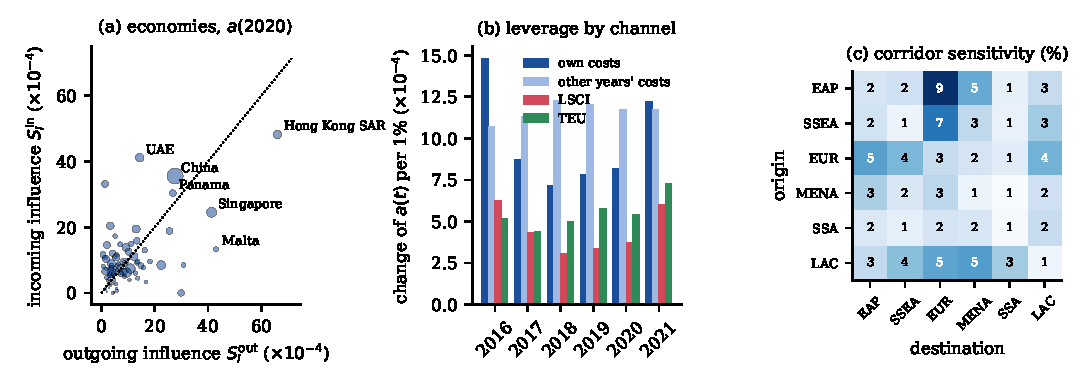
\includegraphics[width=\textwidth]{figures/fig6_sensitivity.pdf}
\caption{(a) Outgoing and incoming influence of each economy on $a(2020)$ (log-cost scale; marker area proportional to mass). (b) Leverage of a 1\% change by channel and year. (c) Share of the corridor sensitivity of the anomaly scores by origin and destination region, averaged over 2016--2021 (\%).}\label{fig:sens}
\end{figure}

\begin{table}[hp]
\caption{Sensitivity of the regional lead--lag indices. $\hat\tau_{\beta/2}$, $\hat\tau_{2\beta}$: index with the temperature halved and doubled. Leading economies: largest total influence on $\hat\tau$ within each region. $\rho$: Spearman correlation of $|\nabla\hat\tau|$ with its value at the main temperature. Abbreviations as in Table~\ref{tab:reg}.}\label{tab:regsens}
\centering\scriptsize
\begin{tabular}{llrrrrllrr}
\toprule
 & & & & & & \multicolumn{2}{c}{leading economy for $\hat\tau$} & \multicolumn{2}{c}{$\rho$}\\
\cmidrule(lr){7-8}\cmidrule(lr){9-10}
$a$ & $b$ & $\hat\tau$ & $\hat\tau_{\beta/2}$ & $\hat\tau_{2\beta}$ & $\widehat{\mathrm{GSTA}}$ & in $a$ & in $b$ & $\beta/2$ & $2\beta$\\
\midrule
EAP & SSEA & +0.95 & +0.97 & +0.91 & 0.260 & Hong Kong SAR & Singapore & 0.99 & 1.00\\
EAP & EUR & $-$0.08 & $-$0.08 & $-$0.12 & 0.546 & Hong Kong SAR & Russian Fed. & 0.99 & 0.98\\
EAP & MENA & +0.06 & +0.03 & +0.11 & 0.606 & Hong Kong SAR & UAE & 1.00 & 0.99\\
EAP & SSA & +0.88 & +0.46 & +1.10 & 1.142 & Hong Kong SAR & Mauritius & 0.96 & 0.96\\
EAP & LAC & $-$0.02 & $-$0.01 & +0.05 & 0.909 & Hong Kong SAR & Panama & 0.96 & 0.95\\
SSEA & EUR & $-$0.95 & $-$0.65 & $-$1.10 & 0.198 & Philippines & Russian Fed. & 0.93 & 0.96\\
SSEA & MENA & +0.28 & +0.31 & +0.36 & 0.176 & Philippines & UAE & 0.99 & 0.98\\
SSEA & SSA & +1.53 & +1.61 & +1.43 & 0.816 & Philippines & Mauritius & 0.98 & 0.98\\
SSEA & LAC & +0.28 & +0.06 & +0.66 & 0.406 & Philippines & Panama & 0.98 & 0.93\\
EUR & MENA & +0.14 & +0.26 & +0.03 & 0.156 & Russian Fed. & UAE & 0.99 & 0.99\\
EUR & SSA & +1.67 & +1.83 & +1.48 & 0.819 & Germany & Mauritius & 0.97 & 0.98\\
EUR & LAC & +1.36 & +1.41 & +1.26 & 0.285 & Malta & Panama & 1.00 & 0.99\\
MENA & SSA & +1.41 & +1.38 & +1.37 & 0.416 & UAE & Togo & 0.98 & 0.99\\
MENA & LAC & +0.64 & +0.49 & +0.80 & 0.089 & UAE & Panama & 0.96 & 0.97\\
SSA & LAC & $-$1.65 & $-$1.84 & $-$1.45 & 0.242 & Mauritius & Panama & 0.99 & 0.99\\
\bottomrule
\end{tabular}
\end{table}

\begin{table}[hp]
\caption{Counterfactual perturbations of corridor costs ($|u_{ik}|\le0.5$ in log cost, budget $B=\sum|u_{ik}|$; knapsack strategies change $2B$ corridors). (i) Relative change of $\Delta(G_{2020},G_{2021})$ when the 2021 costs are perturbed. (ii) Margin $a(2020)-\max_{t\ne2020}a(t)$ (baseline $-0.025$) when the 2020 costs are perturbed, and the smallest budget on the grid $\{8,32,128,512,1024,2048\}$ at which 2020 ranks first. (iii) $\hat\tau(\mathrm{EAP},\mathrm{SSEA})$ (baseline 0.954) when the SSEA costs of all years are perturbed. Random: mean over 5, 2 and 3 draws. All values re-solved with the portfolio.}\label{tab:cf}
\centering\scriptsize
\begin{tabular}{lrrrrrrrrr}
\toprule
 & \multicolumn{3}{c}{(i) change of $\Delta$, \%} & \multicolumn{4}{c}{(ii) margin after} & \multicolumn{2}{c}{(iii) $\hat\tau$ after}\\
\cmidrule(lr){2-4}\cmidrule(lr){5-8}\cmidrule(lr){9-10}
Strategy & $B=8$ & $B=32$ & $B=128$ & $B=128$ & $B=512$ & $B=2048$ & first at $B$ & $B=8$ & $B=16$\\
\midrule
gradient & $-5.3$ & $-12.0$ & $-23.3$ & $+0.0003$ & $+0.0171$ & $+0.0276$ & 128 & 0.818 & 0.769\\
cost-change & $-0.5$ & $-2.8$ & $-9.8$ & $-0.0174$ & $-0.0073$ & $+0.0093$ & 2048 & -- & --\\
mass-weighted & $-0.0$ & $-0.5$ & $-1.7$ & $-0.0141$ & $-0.0017$ & $+0.0225$ & 1024 & 0.931 & 0.916\\
random & $-0.1$ & $-0.2$ & $-1.1$ & $-0.0225$ & $-0.0160$ & $+0.0107$ & 2048 & 0.945 & 0.935\\
uniform & $-0.2$ & $-0.7$ & $-2.8$ & $-0.0237$ & $-0.0192$ & $+0.0046$ & 2048 & 0.944 & 0.933\\
\bottomrule
\end{tabular}
\end{table}

\begin{figure}[t]
\centering
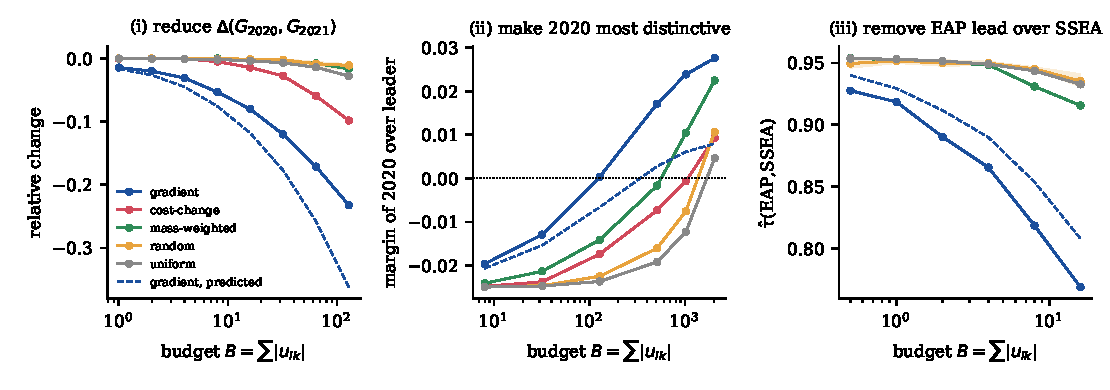
\includegraphics[width=\textwidth]{figures/fig7_counterfactual.pdf}
\caption{Counterfactual perturbations: re-solved values by strategy and budget (solid; random: mean and range over draws) and first-order predictions of the gradient strategy (dashed). (i) Relative change of $\Delta(G_{2020},G_{2021})$. (ii) Margin of 2020 over the leading year; above the dotted line 2020 is the most distinctive year. (iii) $\hat\tau(\mathrm{EAP},\mathrm{SSEA})$.}\label{fig:cf}
\end{figure}

%%%%%%%%%%%%%%%%%%%%%%%%%%%%%%%%%%%%%%%%%%%%%%%%%%%%%%%%%%%%%%%%%%%%%%%%%%%%%%

%============================================================================================
% [M8a] Discussion: insert a new paragraph before the paragraph starting 'Several limitations remain.'
% ANCHOR: Several limitations remain.
% MODE:   insert BEFORE the anchor
%============================================================================================
The sensitivity layer turns G-STA from a measurement into a diagnostic. Because the reported discrepancies are debiased, so must be their derivatives. Gradients of the raw value misstate corridor sensitivities by 5\%--18\% in the application and do not vanish when a state is compared with a copy of itself. The trajectory-level gradient weights state-level gradients by expected alignment frequencies, and the gradient of the lead--lag index is a covariance over alignment paths, which explains why timing sensitivity disappears at zero temperature. First-order predictions identified effective perturbations far beyond the range in which they were accurate in magnitude. Realized changes were 64\%--87\% of predicted reductions of a discrepancy and 125\%--159\% of predicted increases, as the curvature of the re-optimized value implies, and no perturbation changed the selected branch. The counterfactual exercises say which feasible changes of the inputs would move the measured quantities, not what an intervention would achieve in the transport market.

%============================================================================================
% [M8b] Discussion, limitations paragraph: append at its end (after '... remains open.')
% ANCHOR: in the spirit of \citet{sommerfeld2018inference} remains open.
% MODE:   insert AFTER the anchor
%============================================================================================
 The sensitivity results are local and conditional on fixed masks, fixed standardization constants and the selected branches; changes of the observation pattern require re-solving rather than gradients, and the delta-method uncertainty statements rest on an assumed model of independent cost errors.
